\section{Peta Karnaugh 2 Variabel}

Peta Karnaugh 2 variabel merupakan bentuk K-Map yang paling sederhana, terdiri dari $2^2 = 4$ sel yang merepresentasikan seluruh kombinasi input dari dua variabel Boolean. Meskipun sederhana, K-Map 2 variabel sangat berguna sebagai sarana pembelajaran karena memungkinkan mahasiswa memahami konsep-konsep dasar pengelompokan dan eliminasi variabel sebelum melangkah ke K-Map dengan lebih banyak variabel \cite{rosen2019}.

\subsection{Struktur K-Map 2 Variabel}

K-Map 2 variabel disusun sebagai grid $2 \times 2$. Satu variabel digunakan sebagai label baris (misalnya $X$) dan variabel lainnya sebagai label kolom (misalnya $Y$). Setiap sel berkorespondensi dengan satu minterm, sebagaimana ditunjukkan pada Gambar~\ref{fig:kmap-2var}.

\begin{figure}[htbp]
\centering
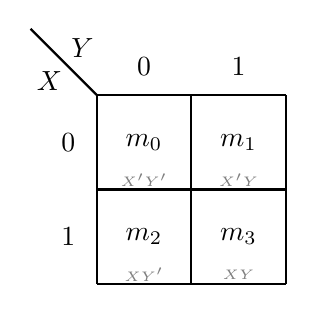
\begin{tikzpicture}[scale=1.2]
    % Grid 2x2
    \draw[thick] (0,0) grid (2,2);
    % Diagonal divider
    \draw[thick] (0,2) -- (-0.7,2.7);
    \node at (-0.5, 2.15) {$X$};
    \node at (-0.15, 2.5) {$Y$};
    % Labels
    \node at (0.5, 2.3) {$0$}; \node at (1.5, 2.3) {$1$};
    \node at (-0.3, 1.5) {$0$}; \node at (-0.3, 0.5) {$1$};
    % Cells with minterm labels
    \node at (0.5, 1.5) {$m_0$}; \node at (1.5, 1.5) {$m_1$};
    \node at (0.5, 0.5) {$m_2$}; \node at (1.5, 0.5) {$m_3$};
    % Small labels for minterms
    \node[font=\tiny, gray] at (0.5, 1.1) {$X'Y'$}; \node[font=\tiny, gray] at (1.5, 1.1) {$X'Y$};
    \node[font=\tiny, gray] at (0.5, 0.1) {$XY'$}; \node[font=\tiny, gray] at (1.5, 0.1) {$XY$};
\end{tikzpicture}
\caption{Struktur Peta Karnaugh 2 Variabel}
\label{fig:kmap-2var}
\end{figure}

Pada K-Map 2 variabel, sel $m_0$ (pojok kiri atas) merepresentasikan kondisi $X = 0, Y = 0$ (minterm $X'Y'$), dan seterusnya. Perhatikan bahwa sel-sel yang bersebelahan secara horizontal berbeda pada variabel $Y$, sedangkan sel-sel yang bersebelahan secara vertikal berbeda pada variabel $X$.

\subsection{Aturan Pengelompokan}

Pengelompokan (\textit{grouping}) merupakan inti dari metode K-Map. Aturan-aturan pengelompokan berlaku sama untuk K-Map dengan jumlah variabel berapa pun, dan ditetapkan sebagai berikut \cite{wiki_karnaugh}:

\begin{enumerate}[label=\textbf{R\arabic*.}]
  \item \textbf{Ukuran kelompok harus pangkat dua}: Kelompok harus berisi $2^k$ sel (yaitu 1, 2, atau 4 sel pada K-Map 2 variabel).
  \item \textbf{Bentuk persegi panjang}: Kelompok harus berbentuk persegi atau persegi panjang (tidak boleh diagonal atau bentuk L).
  \item \textbf{Maksimalkan ukuran}: Setiap kelompok harus dibuat sebesar mungkin untuk memaksimalkan jumlah variabel yang dieliminasi.
  \item \textbf{Minimalkan jumlah kelompok}: Gunakan jumlah kelompok seminimal mungkin untuk mencakup seluruh sel bernilai 1.
  \item \textbf{Semua sel bernilai 1 harus tercakup}: Setiap sel yang bernilai 1 harus masuk ke dalam setidaknya satu kelompok.
  \item \textbf{Tumpang tindih diperbolehkan}: Kelompok boleh saling tumpang tindih (\textit{overlap}) jika hal itu menghasilkan kelompok yang lebih besar.
\end{enumerate}

\subsection{Eliminasi Variabel}

Setelah kelompok terbentuk, variabel yang berubah nilainya di dalam kelompok tersebut dieliminasi. Variabel yang tetap konstan di seluruh sel dalam kelompok menjadi bagian dari suku hasil penyederhanaan. Jumlah variabel yang dieliminasi bergantung pada ukuran kelompok:

\begin{center}
\renewcommand{\arraystretch}{1.2}
\begin{tabular}{|c|c|c|}
\hline
\textbf{Ukuran Kelompok} & \textbf{Variabel Dieliminasi} & \textbf{Suku Hasil} \\ \hline
1 sel & 0 variabel & Minterm lengkap \\ \hline
2 sel & 1 variabel & Suku dengan $(n-1)$ literal \\ \hline
4 sel & 2 variabel & Suku dengan $(n-2)$ literal \\ \hline
$2^k$ sel & $k$ variabel & Suku dengan $(n-k)$ literal \\ \hline
\end{tabular}
\end{center}

\subsection{Contoh Penyederhanaan K-Map 2 Variabel}

\begin{contoh}
\textbf{Penyederhanaan $F(X,Y) = \sum m(0, 1, 3)$}

\textbf{Langkah 1:} Tempatkan nilai 1 pada sel $m_0$, $m_1$, dan $m_3$:

\begin{center}
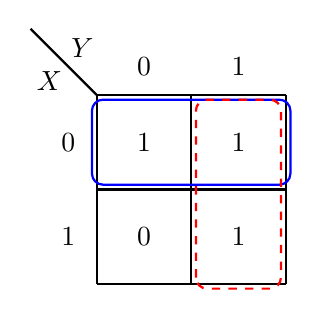
\begin{tikzpicture}[scale=1.2]
    \draw[thick] (0,0) grid (2,2);
    \draw[thick] (0,2) -- (-0.7,2.7);
    \node at (-0.5, 2.15) {$X$};
    \node at (-0.15, 2.5) {$Y$};
    \node at (0.5, 2.3) {$0$}; \node at (1.5, 2.3) {$1$};
    \node at (-0.3, 1.5) {$0$}; \node at (-0.3, 0.5) {$1$};
    % Values
    \node at (0.5, 1.5) {1}; \node at (1.5, 1.5) {1};
    \node at (0.5, 0.5) {0}; \node at (1.5, 0.5) {1};
    % Group 1: top row
    \draw[thick, blue, rounded corners] (-0.05, 1.05) rectangle (2.05, 1.95);
    % Group 2: right column
    \draw[thick, red, rounded corners, dashed] (1.05, -0.05) rectangle (1.95, 1.95);
\end{tikzpicture}
\end{center}

\textbf{Langkah 2:} Identifikasi kelompok:
\begin{itemize}
    \item \textcolor{blue}{Kelompok 1 (biru)}: $\{m_0, m_1\}$ --- baris atas, $X = 0$ konstan, $Y$ berubah $\Rightarrow$ suku: $X'$
    \item \textcolor{red}{Kelompok 2 (merah)}: $\{m_1, m_3\}$ --- kolom kanan, $Y = 1$ konstan, $X$ berubah $\Rightarrow$ suku: $Y$
\end{itemize}

\textbf{Langkah 3:} Hasil penyederhanaan: $F = X' + Y$

\textbf{Verifikasi aljabar:}
\begin{align*}
F &= \sum m(0, 1, 3) = X'Y' + X'Y + XY \\
  &= X'(Y' + Y) + XY = X' + XY \\
  &= X' + Y \quad \text{(absorpsi: } X' + XY = X' + Y)
\end{align*}

Hasil K-Map dan hasil aljabar cocok: $F = X' + Y$.
\end{contoh}
